\section{Microfrontends}

With the introduction of the \gls{ma} pattern, \gls{backend} systems can be
split up into multiple services, each with their own responsibilities. As
previously described, this can bring great benefit. However, even after a
transition to \glsplural{microservice} on the server-side, the client-side
applications using these services are mostly still \gls{monolithic} in nature.

A \gls{monolithic} \gls{frontend} does not have to be a problem.
\Glsplural{monolith} are quick and easy to set up, and historically, most of the
heavy lifting was done on the server-side anyway. However, the complexity of
client-side applications has seen a drastic increase over the last few years.
This can be attributed to many factors: increased hardware and web browser
capabilities, a broad variety of client devices, a massive market growth for
digital services, and the web transitioning from a document platform to the
largest application platform \autocite{Ball_2019}, just to name a few.

In these complex applications, the downsides of a \gls{monolithic} architecture
come back into view: every change requires the entire \gls{frontend} application
to be rebuilt and redeployed, codebases grow very large in size, etc... Even
worse, because the client-side application has a functional dependency on the
server-side application, a small change in one particular area of the
\gls{backend} logic could also trigger a change in the \gls{frontend}, causing
the entire \gls{frontend} to yet again be rebuilt and redeployed
\autocite{Rappl_LogRocket_2019}.

There's also the issue of \textbf{domain knowledge}: while the \gls{ma} gives
\gls{backend} teams the possibility of focussing on one specific part of a
business domain, teams that are developing the client-side code are still
expected to know the entire scope of the application. Often this means a
reliance on personal inter-team communication, which in larger organizations
tends to be expensive \autocite{Geers_2020}. 

While component-based paradigms introduced by libraries and frameworks (such as
React\hreffootnote{https://reactjs.org},
Angular\hreffootnote{https://angular.io} and
Vue\hreffootnote{https://vuejs.org}) can aliviate some of the complexity of the
current frontend systems, they still do not enable  fully autonomous, decoupled,
modular and/or distributed development of large web applications.

\subsection{What are microfrontends?}

In 2016 the ThoughtWorks Technology Radar \autocite{ThoughtWorks_2020} coined
the term ``\textit{Micro Frontends}'' to describe the split of the
\gls{frontend} \gls{monolith} into independently deployable and maintainable
pieces. This new architecture pattern could therefore be regarded as an
extension of the \gls{ma} into the \gls{frontend} space.

The characteristics of the \gls{mfa} pattern are therefore very closely related
to those of the \gls{ma} pattern, as described in section
\fullref{principles-of-the-mfa}. Every individual \gls{frontend} module has a
relatively small codebase, is focussed around one specific domain or company
mission, and should be modular, decoupled and independently developed; most
optimally by autonomous teams.

A visual represtation of the \gls{mfa} pattern is shown in
Figure~\ref{fig:microfrontends}.


\begin{figure}
  \centering
  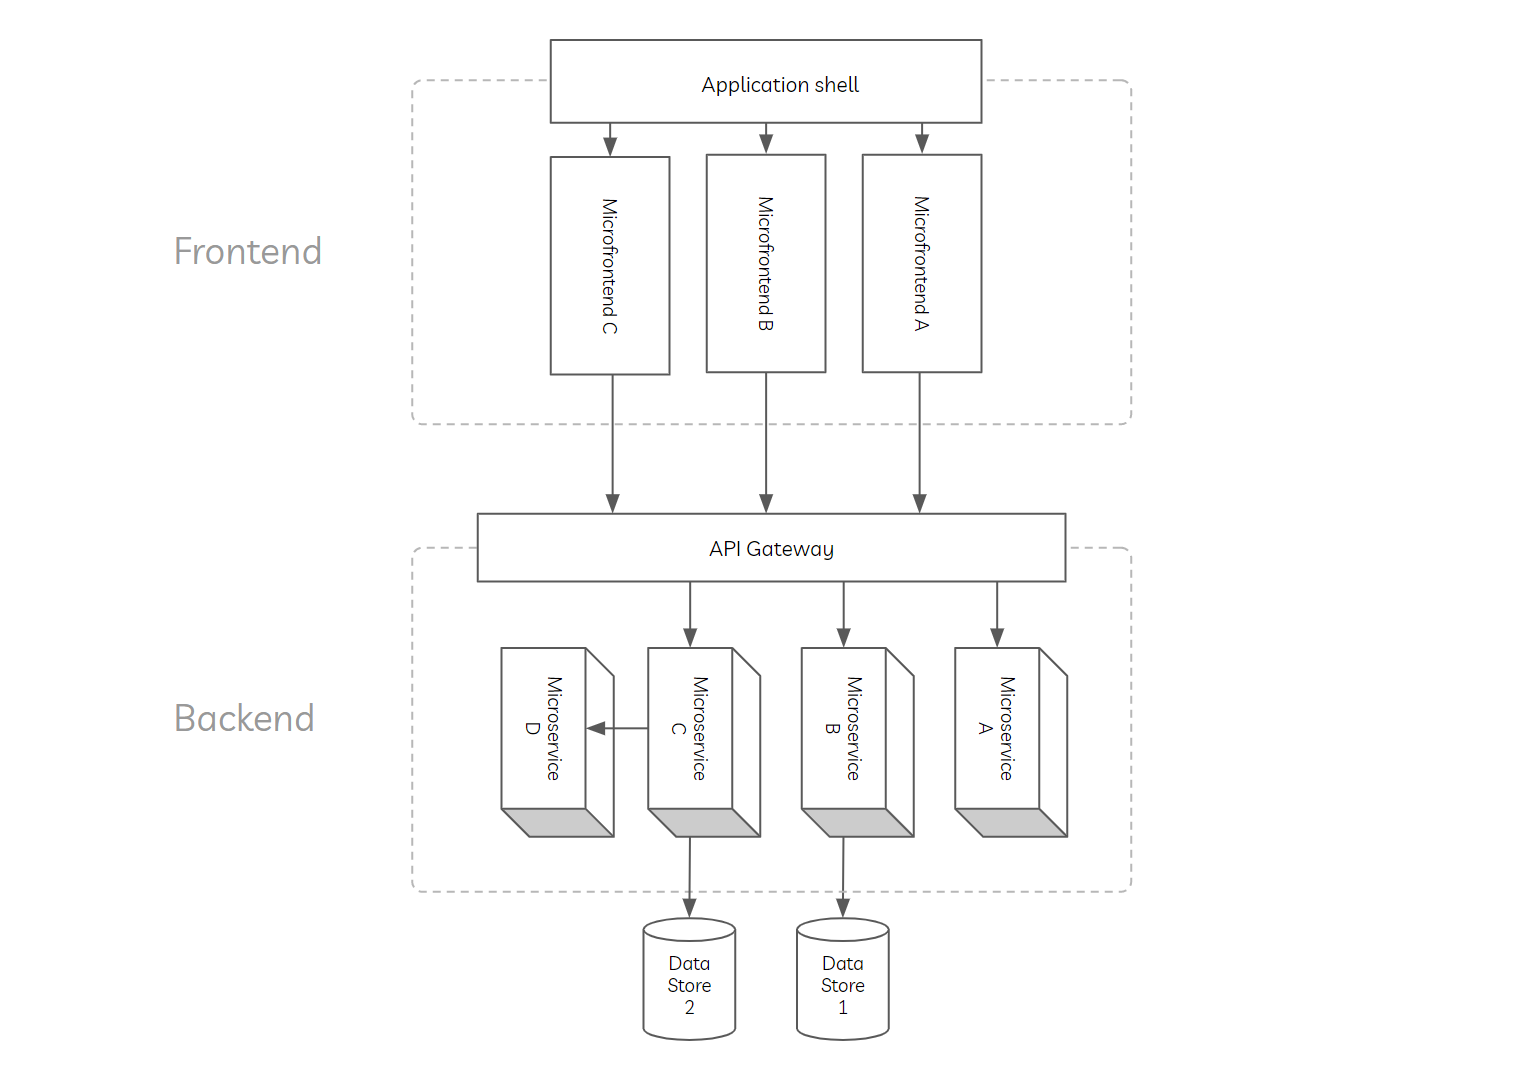
\includegraphics[width=\textwidth]{microfrontends.png}
  \caption[Microfrontends]{A diagram showing an example of a
  \gls{mfa}.}
  \label{fig:microfrontends}
\end{figure}

\subsection{How do microfrontends enable distributed development?}

A significant difference between \glsplural{microfrontend} and other software
architectures is the impact on \textbf{team structure} and organizational shift
\autocite{Geers_2020}.

So, while \glsplural{microfrontend} have lots of technical aspects to consider,
it is important to reflect on the organizational aspects first.

As disussed in \fullref{ssec:microservices}, when adopting the \gls{ma}, a shift
has to be made to smaller independent teams around a specific business need.
However, this only brings about changes in the \gls{backend} teams, while the
\gls{frontend}-oriented development team will usually not follow suit. This
keeps the overarching team structure ``horizontal'': divided per layer or
technology.

One of the benefits of horizontal teams is that this structure enables experts
focussing on specific technologies to co-operate together as one team. This way
they can ensure a high technical standard within the boundaries of their
respective areas of expertise.

In geographically distributed teams, the consequence could be that these
technical teams operate from entirely different locations. According to
\textcite{Smite_etal_2010}, this can result in compatibility issues between software
layers and a less customer-focused development model. Moreover, disputes can
arise between the different teams because no team has full responsibility over
the delivery of any feature.

\subsubsection{Feature teams}
\label{feature-teams}

%TODO add images?

To mitigate the issues arising from geographically distributed horizontal teams;
multidisciplinary or cross-functional ``feature teams'' can be introduced. These
are grouped around a specific business case or customer need. This ``vertical
slicing''  enables teams to be more independent and have end-to-end
responsibility for the features they develop.

This feature team approach has multiple advantages: \autocite{Smite_etal_2010}
\begin{itemize} 
  \item \textbf{Optimized feature development}\\
  Focussing on features in stead of technical details aids in delivering the
  highest amount of business value.
  % 
  \spacedItem \textbf{Decreased need for ``expensive'' communication}\\
  Communications within a team is usually faster and more informal than
  communications between teams, especially if teams are geographically
  distributed. Since a feature can be developed by a single team, the need for
  expensive communication decreases.
  %
  \spacedItem \textbf{Greater sense of developer involvement}\\
  According to \autocite{LarmanVodde_2008}, developers who operate in a feature
  team feel a greater sense of ownership and accountability for the features
  they develop. 
  %
\end{itemize}

It is worth mentioning that these benefits combined can result in a faster cycle
time and thus an increase in development speed \autocite{Geers_2020}.

On the other side, this approach also comes with caveats. One of them is the
danger of compromising on the \textbf{conceptual integrity} of the software
systems. More time will have to be spent up-front laying a solid foundation for
conventions and standards. The effort to then maintain the consistency of the
software system is usually where the software architect has a key role. In
larger projects, a technical service team can be assembled to provide technical
coherence across different distributed systems \autocite{Smite_etal_2010}. WHile
this is something to consider, this also means an increased emphasis on better
code quality right from the start, which could prove very beneficial in the long
term \autocite{LarmanVodde_2008}.

Another caveat is that, especially in large corporations, \textbf{changing the
complicated organizational structure} might not be possible, or at the very
least slow and difficult.

\subsection{Common implementation patterns}
\label{ssec:mf-implementation-patterns}

As is the case with lots of architectural patterns, there are many ways of
implementation possible. With the \gls{mfa}, this is no different. Various
options differ in complexity, goal, and mechanism. 

\Gls{microfrontend} often need to be composed to be able to reach a coherent
application. Every microfrontend brings it's own \textbf{pages}. Often,
\glsplural{microfrontend} also expose reusable components to be rendered in a
variety of locations, to provide functionality. These are often called
\textbf{fragments}.

Below some of the possible implementation and composition techniques are
outlined.

\subsubsection{The \textit{web approach}}

The most straightforward way of leveraging the \gls{mfa} pattern is by not using
any integration technique at all. In stead, there can be opted for mechanisms
that exist in the world of the web. 

As described by \textcite{Rappl_2021}, the \textit{web approach}'s main approach
for \gls{microfrontend} referencence is by way of their \gls{url}.
\textbf{Hyperlinks} can be used to let the user navigate between different
\glsplural{microfrontend}. This however compromises on user experience and
usability. With this approach, for example, elements from multiple
\glsplural{microfrontend} cannot be rendered on the same page. 

To enable visual composition of \glsplural{microfrontend} in the most
straightforward way, \textbf{\glsplural{iframe}} can be used. By using an
\texttt{<iframe>} tag with a \texttt{src} attribute that points to a \gls{url},
one could embed visual components of one \gls{microfrontend} within another,
without sacrificing on strong isolation between the two \autocite{Geers_2020}.
The disadvantage here is the notoriously bad characteristics of
\glsplural{iframe}. One of these is bad performance: according to
\textcite{Souders_2013}, \glsplural{iframe} are up to 2 orders of magnitude more
expensive to create than any other \gls{dom} element. Moreover, iframes also
block the loading process of the rest of the page. Other suboptimal
characteristics include accessibility and \gls{seo}.

The simplicity of the web approach is also where it lacks applicability for
larger projects. One of the biggest reasons to implement
\glsplural{microservice} and \glsplural{microfrontend} is scalibility, which the
web approach is often not very suitable for.

\subsubsection{Server-side composition}

To accomodate for scalibility and esure higher performance, the composition of
the \glsplural{microfrontend} can be done before even reaching the end user's
web browser. This will require dynamically composing the application on the
server side.

According to \textcite{Geers_2020}, this server-side composition can also
provide a solid basis to be able to enable \gls{pe}, and is a big advantage for
\gls{seo}.

There are multiple techniques to enable server-side composition. These include,
but are not limited to:
\begin{itemize}
  \item \textbf{\gls{ssi}}.\\
  This uses an \textit{\gls{ssi} directive} (a HTML comment) to signify a
  placeholder for fragments to be rendered into.
  \begin{minted}{html}
<!-- #include virtual="/fragment" -->
  \end{minted}
  It also support the execution of commands from the server, and even some
  conditional logic \autocite{Apache_2013}. \gls{ssi} has been around for a long
  time, this way most web servers have support for it. Because its directives
  are HTML comments, using these on a server that is not configured for
  \gls{ssi} won't crash the application (the fragment will just simply not be
  rendered).
  %
  \spacedItem  \textbf{\gls{esi}}.\\
  In stead of HTML comments, \gls{esi} uses \gls{xml}-based \gls{esi} tags:
  \begin{minted}{xml}
<esi:include  src="/fragment" 
              alt="/fallback" 
              onerror="continue" />
  \end{minted}
  \gls{esi} has a more extensive amount of functionalities (error handling,
  fallbacks, ...) compared to \gls{ssi}. It is however more difficult to
  implement \autocite{Rappl_2021}.
\end{itemize}


\subsubsection{Client-side composition}

While with server-side composition, a web server was used as an aggregation
layer for integrating the \glsplural{microfrontend}; with client-side
composition the goal is to put this responsibility onto the end user's browser
itself. The browser will have to render one parent HTML document which contains
the instructions to integrate all the individual \glsplural{microfrontend} into
itself.

This parent HTML document is often called the \textbf{\gls{appshell}}
\autocite{Geers_2020}\autocite{Rappl_2021}. 

The \gls{microfrontend} scripts and resources are often served from a
\textbf{\gls{cdn}}.

Client-side composition can be done in various different ways. A selection is
outlined below:
\begin{itemize}
  \item \textbf{Web Components}\\
  According to \textcite{Mozilla_WebComponents}, this term encompasses three
  main technologies, namely custom elements, shadow \gls{dom} (that can provide
  reusable \gls{dom} trees to ensure isolation) and HTML templates.
  % 
  \spacedItem \textbf{\gls{spa} composition}\\
  In recent years, client-side frameworks have become the staple of fast and
  app-like experiences on the web. Most of these frameworks introduce a custom
  client-side routing solution. When using \gls{spa} composition, the app shell
  needs to take responsibility for the routing. The \gls{appshell} will now not
  just render fragments using HTML, but execute scripts defined in the
  \glsplural{microfrontend} themselves to be able to integrate them.
\end{itemize}

Client-side composition is great for delivering highly interactive, dynamic web
applications. However, because the application is not served to the browser in
full, the downsides include suboptimal \gls{seo} and a increased time to first
load.

\subsubsection{Universal composition}
\label{sssec:universal-composition}

Aiming to combine the client-side and server-side composition approaches, and
get the advantage of both, a hybrid approach can be achieved. Universal -- or
\textit{isomorphic} -- composition describes the process of 
\begin{enumerate}
  \item composing the application on the server side, providing a fast initial
  load and thus enabling \gls{pe} and optimal \gls{seo}
  \item \textit{hydrating} the application so it becomes fully client-side
  interactive, providing the benefits of a highly dynamic application.
\end{enumerate}


\subsection{Usage of microfrontends}

\Glsplural{microfrontend} are being used by companies all over the world.
Swedish furniture company IKEA mainly uses autonomous vertical teams that can
develop in different technologies if necessary \autocite{Stenberg_2018}.
Spotify, a music streaming service provider from that same country, uses
\gls{iframe}-based \glsplural{microfrontend} within its desktop application to
be able to develop different parts from the same view independently. These
so-called \textit{Spotlets} are developed by \textit{Squads}, independent
cross-functional teams \autocite{Gall_2018}. German e-commerce fashion retailer
Zalando even created ``Project Mosaic''\hreffootnote{https://www.mosaic9.org/},
which contains a plethora of libraries and services to create both
\gls{frontend} and \gls{backend} \glsplural{microservice}.



\subsection{Benefits of microfrontends}

The \gls{mfa} carries over a lot of the advantages of the \gls{ma}
\autocite{Jackson_2019}: \textbf{technology independence} is now also possible
across different \gls{frontend} teams, allowing them to select the best tools
and frameworks for the job. Loose coupling enables the \textbf{scalibility} of
both the \gls{frontend} and \gls{backend}. Now, the \gls{frontend} can also
enjoy the benefits of independent deploys, isolated risks, and smaller
codebases.

\textbf{Teams} also benefit greatly and can be reorganized to even greater
benefit, as was discussed in detail in section \fullref{feature-teams}.

These factors can have great results for a business. Due to their loose
coupling, isolated features and independent deployments,
\glsplural{microfrontend} can have vastly different release cycles, and
iteration and \textbf{feature development} is usually faster because the teams
don't have to wait for each other \autocite{Geers_2020}. \textcite{Rappl_2021},
because there is an existing composition mechanism, different
\glsplural{microfrontend} can be served to different users, enabling the
introduction of \textbf{A/B testing} without significant changes in the
\glsplural{microfrontend} themselves.

\subsection{Downsides and challenges of microfrontends}

However, to use the words of Cam \textcite{Jackson_2019}: \textit{``there are no
free lunches when it comes to software architecture - everything comes with a
cost''}. The \gls{mfa} does indeed come with a significant amount of tradeoffs
that need to be considered. 

\textbf{Organizational complexity} might be one of the biggest downsides of the
\gls{microfrontend} approach. This makes \glsplural{microfrontend} harder to
recommend to small development teams and companies. \textbf{Domain decoposition}
is often difficult and relies on a lot of organizational and technical factors. 

\textbf{Operational complexity} also increases: debugging, logging,
monitoring... all get a lot more complicated. Communication between the
different \glsplural{microfrontend} is generally also way more complex. If the
\gls{microfrontend} solution introduces the need for an \gls{appshell}, this
needs to be closely managed since it introduces a new single point of failure.

Lastly, lots of challenges are inherited from the \gls{ma}, as described in
\textit{``\nameref{sssec:microservice-challenges}''}.

